\documentclass[11pt]{amsart}
\usepackage[margin=1in]{geometry}
\usepackage{amsmath,amssymb,amsthm,booktabs,microtype}
\usepackage{tikz}
\usepackage[colorlinks=true,linkcolor=blue,urlcolor=blue,citecolor=blue,
hypertexnames=false]{hyperref}

\newtheorem{theorem}{Theorem}
\newtheorem{lemma}[theorem]{Lemma}
\newtheorem{remark}[theorem]{Remark}
\newcommand{\Sph}{\mathbb S^2}
\newcommand{\cP}{\mathcal P}

\title{Negative Riesz energies of the BEMOC point set\\
and the sum of mutual distances}
\author{}
\date{28 July 2026}

\begin{document}
\begin{abstract}
Let $\cP_N\subset\mathbb S^2$ be the explicit point set of Beltr\'an,
Etayo, Marzo and Ortega-Cerd\`a.  For every $0<\alpha<2$ we prove
\[
 \sum_{\substack{x,y\in\cP_N\\x\ne y}}|x-y|^\alpha
 =\frac{2^{\alpha+1}}{\alpha+2}N^2
   -\Theta_\alpha\bigl(N^{1-\alpha/2}\bigr).
\]
Thus one explicit family has the optimal second-order scale simultaneously
for all negative Riesz parameters $-2<s<0$.  In particular, at $\alpha=1$,
\[
 \sum_{x\ne y}|x-y|=\frac43N^2-\Theta(\sqrt N),
\]
which settles the sum-of-distances problem for this configuration.  We also
compute the
within-ring contribution: along $N=4m^2$, its normalized limit is
\[
 -\kappa_\alpha(4\pi)^\alpha\zeta(-\alpha),\qquad
 \kappa_\alpha=
 \left[\left(\frac83\right)^{1-\alpha}
       +\left(\frac43\right)^{1-\alpha}\right]
 \frac{2^{1+\alpha/2}-1}{\alpha+2},
\]
where $\zeta$ is the Riemann zeta function.  The latitude and cross-ring
terms generally occur on the same scale, so this is not asserted to be the
coefficient of the full energy.
\end{abstract}
\maketitle

\section{Introduction and statement}

For $0<\alpha<2$ define the maximal distance-power energy
\[
 \mathcal M_\alpha(N)=\max_{\#X=N}
 \sum_{\substack{x,y\in X\\x\ne y}}|x-y|^\alpha.
\]
The continuous energy of normalized surface area $\sigma$ is
\begin{equation}\label{eq:continuous}
 I_\alpha:=\iint_{\Sph\times\Sph}|x-y|^\alpha
 \,d\sigma(x)d\sigma(y)=\frac{2^{\alpha+1}}{\alpha+2}. \tag{1.1}
\end{equation}
Indeed, for fixed $x\in\Sph$ the variable $u=x\cdot y$ is uniform on
$[-1,1]$ under $d\sigma(y)$, and hence
\[
 I_\alpha=\frac12\int_{-1}^1(2-2u)^{\alpha/2}\,du
 =\frac14\int_0^4v^{\alpha/2}\,dv
 =\frac{2^{\alpha+1}}{\alpha+2}.
\]
Since $|x-y|^\alpha$ is a conditionally negative definite kernel,
$\sum_{x\ne y}|x-y|^\alpha\le I_\alpha N^2$.  The classical estimates of
Wagner, summarized in \cite[Theorem~3.6]{HMS}, give
\begin{equation}\label{eq:optimalorder}
 I_\alpha N^2-\mathcal M_\alpha(N)\asymp_\alpha
 N^{1-\alpha/2}.                                     \tag{1.2}
\end{equation}
The conjecture of Brauchart--Hardin--Saff predicts a limiting coefficient
expressed through the triangular-lattice Epstein zeta function
\cite{BHS}.  That coefficient is not known in general.

The case $\alpha=1$ has an additional discrepancy interpretation.
Stolarsky's invariance principle \cite{Stolarsky} identifies
\[
 \frac43N^2-\sum_{x\ne y}|x-y|
\]
with four times $N^2$ times the squared spherical-cap $L^2$ discrepancy.
Together with Beck's sharp discrepancy estimates \cite{Beck}, this gives the classical
extremal result
\[
 \max_{\#X=N}\sum_{x\ne y\in X}|x-y|
 =\frac43N^2-\Theta(\sqrt N).
\]
The expected refinement of Brauchart--Hardin--Saff is
\[
 \max_{\#X=N}\sum_{x\ne y\in X}|x-y|
 =\frac43N^2-c_*\sqrt N+o(\sqrt N),
 \qquad
 c_*=-\left(\frac{8\pi}{\sqrt3}\right)^{1/2}
 \zeta_\Lambda(-1)=0.79851125\ldots,
\]
where $\Lambda$ is the unit-edge triangular lattice.  Neither existence of
this limit nor the predicted value is known.  Our theorem proves the optimal
order for the explicit BEMOC set; it does not identify its full limiting
coefficient.

\subsection{The BEMOC configuration}

We recall the construction so that the proof is self-contained.  Fix
$N\ge16$ and put
\[
 M=\left\lfloor\sqrt{N/4}\right\rfloor,\qquad
 r_j=4j-1\quad(1\le j<M),\qquad
 r_M=N-2\sum_{j=1}^{M-1}r_j .
\]
Extend symmetrically by $r_{M+j}=r_{M-j}$ for $1\le j<M$, and define
\[
 H_0=1,\qquad H_j=1-\frac2N\sum_{k=1}^jr_k,\qquad
 h_j=\frac{H_{j-1}+H_j}{2}.
\]
For $2\le j\le2M-2$, decompose
$r_j=\widetilde r_j+\operatorname{rem}_j$, where
$6\mid\widetilde r_j$ and $0\le\operatorname{rem}_j\le5$, and use the
endpoint conventions
\[
 \widetilde r_1=\widetilde r_{2M-1}=0,
 \qquad \operatorname{rem}_1=r_1,
 \qquad \operatorname{rem}_{2M-1}=r_{2M-1}.
\]
The occupied
parallels and their populations are
\begin{align*}
 Q_{h_1},Q_{h_{2M-1}} &: r_1,\\
 Q_{h_j}\quad(2\le j\le2M-2)&:
 \frac{4\widetilde r_j}{6}+\operatorname{rem}_j,\\
 Q_{H_j}\quad(1\le j\le2M-2)&:
 \frac{\widetilde r_j+\widetilde r_{j+1}}6.
\end{align*}
Every parallel carries an equally spaced polygon.  We allow its azimuthal
phase to be arbitrary and independent of all the other phases.  The formulas
above are the admissible parameters in Lemma~1.6 of \cite{BEMOC}.
Their cardinality is transparent band by band: the midpoint atom and the
two half-contributions at the boundary atoms have total weight
\[
 \frac{4\widetilde r_j}{6}+\operatorname{rem}_j
 +2\frac{\widetilde r_j}{6}=r_j.
\]
After shared boundary atoms are combined, the total number of points is
$\sum_{j=1}^{2M-1}r_j=N$ by the definition of $r_M$ and the symmetry.

\begin{figure}[t]
\centering
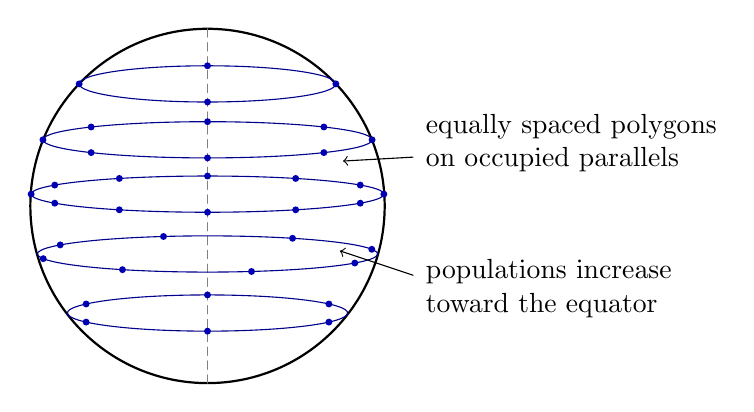
\begin{tikzpicture}[scale=1.0,line cap=round,line join=round]
  \def\R{2.25}
  \draw[thick] (0,0) circle (\R);
  \draw[densely dashed,gray] (0,-\R) -- (0,\R);
  \foreach \y/\rx/\step/\shift in
   {1.55/1.63/90/0,.84/2.09/45/0,.15/2.24/30/0,
    -.61/2.16/45/15,-1.36/1.78/60/30}{
    \draw[blue!55!black] (0,\y) ellipse [x radius=\rx,y radius=.23];
    \foreach \a in {0,\step,...,359}
      \fill[blue!70!black]
       ({\rx*cos(\a+\shift)},{\y+.23*sin(\a+\shift)}) circle (1.25pt);
  }
  \node[align=left,anchor=west] at (2.65,.80)
    {equally spaced polygons\\on occupied parallels};
  \draw[->] (2.61,.62)--(1.72,.57);
  \node[align=left,anchor=west] at (2.65,-1.05)
    {populations increase\\toward the equator};
  \draw[->] (2.61,-.88)--(1.68,-.57);
\end{tikzpicture}
\caption{Schematic BEMOC configuration.  There are $O(\sqrt N)$ occupied
parallels, and the phases of their polygons may be chosen independently.}
\label{fig:bemoc}
\end{figure}

The set lies on $O(\sqrt N)$ parallels.  A ring $p$ has height
$z_p$, radius $\rho_p$, and population $w_p$, with
\begin{equation}\label{eq:geometry}
 w_p\asymp M\rho_p,\qquad M=\lfloor\sqrt{N/4}\rfloor,
 \qquad \sum_p\rho_p\asymp M.                       \tag{1.3}
\end{equation}
The population--radius comparison holds for all occupied rings, after a
fixed enlargement of its constants.  The exceptional equatorial population
will nevertheless be separated in the arithmetic sum because it need not
belong to the affine population families used there.
It follows from $H_j=1-2N^{-1}\sum_{k\le j}r_k$ and $r_j\asymp j$: near a
pole, $1-H_j\asymp j^2/M^2$, so
$\rho_j=\sqrt{1-H_j^2}\asymp j/M$ and $w_j\asymp j$.

\begin{theorem}\label{thm:main}
For each fixed $0<\alpha<2$ there are constants
$0<c_\alpha<C_\alpha<\infty$ such that
\[
 c_\alpha N^{1-\alpha/2}
 \le I_\alpha N^2-
 \sum_{\substack{x,y\in\cP_N\\x\ne y}}|x-y|^\alpha
 \le C_\alpha N^{1-\alpha/2}.
\]
The upper bound is uniform under independent rotations of all polygons.
\end{theorem}

The lower bound follows immediately from \eqref{eq:optimalorder}; the work
is the upper bound for this particular configuration.  We give the proof at
the total-energy level, avoiding any assertion that a neighborhood of a
point is one triangular lattice.

For orientation, the proof inserts continuous angular measure on each
parallel.  The resulting deficit splits into three terms:
\[
 \boxed{\text{latitude quadrature}}
 \; +\; \boxed{\text{within-ring discretization}}
 \; +\; \boxed{\text{cross-ring angular aliasing}}.
\]
Each term is $O_\alpha(N^{1-\alpha/2})$.  The first uses the two exact
moments built into the BEMOC construction, the second is a one-dimensional
Euler--Maclaurin calculation, and the third is a Fourier/gcd estimate.

\section{Ring decomposition}

Let $U_p$ be uniform probability measure on ring $p$ and put
$\nu=\sum_pw_pU_p$.  For heights $s,t$ define
\[
 F_\alpha(s,t)=\frac1{2\pi}\int_0^{2\pi}
 \left(2-2st-2\sqrt{1-s^2}\sqrt{1-t^2}\cos\theta
 \right)^{\alpha/2}d\theta.
\]
Writing $E_\alpha[\nu]=\sum_{p,q}w_pw_qF_\alpha(z_p,z_q)$ and inserting
this continuous angular measure gives the exact decomposition
\begin{equation}\label{eq:decomp}
 D_{\alpha,N}:=I_\alpha N^2-E_\alpha(\cP_N)
 =A_{\alpha,N}+B_{\alpha,N}+C_{\alpha,N},             \tag{2.1}
\end{equation}
where
\begin{align*}
 A_{\alpha,N}&=I_\alpha N^2-E_\alpha[\nu],\\
 B_{\alpha,N}&=\sum_p\left(w_p^2\rho_p^\alpha J_\alpha
                    -\Sigma_{\alpha,p}^{\rm self}\right),\\
 C_{\alpha,N}&=\sum_{p\ne q}\left(w_pw_qF_\alpha(z_p,z_q)
                    -\Sigma_{\alpha,pq}^{\rm cross}\right),
\end{align*}
and
\[
 J_\alpha=\frac1{2\pi}\int_0^{2\pi}
 (2\sin(\theta/2))^\alpha d\theta.
\]
To see the identity directly, first separate the ordered pairs belonging to
one ring from those belonging to two different rings.  On ring $p$, the
continuous angular self-energy is $w_p^2\rho_p^\alpha J_\alpha$; for
$p\ne q$ it is $w_pw_qF_\alpha(z_p,z_q)$.  Adding and subtracting precisely
these quantities produces the three displayed terms, without an error term.

For completeness, Schoenberg's theorem says that $|x-y|^\alpha$ is
conditionally negative definite for $0<\alpha<2$.  Thus, for every signed
measure $\eta$ of total mass zero,
\[
 \iint |x-y|^\alpha\,d\eta(x)d\eta(y)\le0.
\]
Apply this with $\eta=\nu-N\sigma$ and with the point measure minus
$N\sigma$.  Since the potential of $\sigma$ is constant, the cross terms
vanish and we obtain $A_{\alpha,N}\ge0$ and $D_{\alpha,N}\ge0$.

\section{The explicit within-ring term}

\begin{lemma}[endpoint Euler--Maclaurin]\label{lem:circle}
For fixed $0<\alpha<2$,
\begin{equation}\label{eq:circle}
 \sum_{k=1}^{w-1}\left(2\sin\frac{\pi k}{w}\right)^\alpha
 =wJ_\alpha+2(2\pi)^\alpha\zeta(-\alpha)w^{-\alpha}
 +o_\alpha(w^{-\alpha}).                             \tag{3.1}
\end{equation}
The remainder divided by $w^{-\alpha}$ is bounded uniformly for $w\ge2$.
\end{lemma}

\begin{proof}
The function $f(x)=(2\sin\pi x)^\alpha$ has endpoint expansions
\[
 f(x)=(2\pi)^\alpha x^\alpha+O_\alpha(x^{\alpha+2}),
 \qquad f(1-x)=(2\pi)^\alpha x^\alpha+O_\alpha(x^{\alpha+2}).
\]
Here is a little more detail about the endpoint calculation.  Choose a
smooth cutoff $\chi$ supported near zero and equal to one in a smaller
neighborhood, and write
\[
 f(x)=(2\pi)^\alpha\{\chi(x)x^\alpha+
 \chi(1-x)(1-x)^\alpha\}+g(x).
\]
After subtracting also the next endpoint term, of order
$x^{\alpha+2}$, the residual has the ordinary endpoint regularity needed
for the composite Euler--Maclaurin formula.  For the singular model, the
finite-part power-sum expansion is
\[
 \sum_{k=1}^{w-1}k^\alpha
 =\frac{w^{\alpha+1}}{\alpha+1}-\frac12w^\alpha
   +\zeta(-\alpha)+O_\alpha(w^{\alpha-1})
\]
and the same expansion holds at the other endpoint.  After the mesh factor
$w^{-\alpha}$ is restored, the integral terms of the singular pieces and of
$g$ combine to
\[
 w\int_0^1f(x)\,dx=wJ_\alpha.
\]
Their $1/2$-endpoint terms and all ordinary integer-power corrections cancel
as well; this cancellation is important for $1<\alpha<2$, where retaining
only the singular pieces would create a spurious $w^{-1}$ term.  What remains
first is one copy of $(2\pi)^\alpha\zeta(-\alpha)w^{-\alpha}$ from each
endpoint, proving \eqref{eq:circle}.  Subtracting the $x^{\alpha+2}$ terms
before applying Euler--Maclaurin gives a remainder
$O_\alpha(w^{-\alpha-2})$, in particular the uniform domination stated in
the lemma.
\end{proof}

\begin{lemma}\label{lem:within}
$0\le B_{\alpha,N}\le C_\alpha N^{1-\alpha/2}$.  Along $N=4m^2$,
\[
 \frac{B_{\alpha,N}}{N^{1-\alpha/2}}
 \longrightarrow
 -\kappa_\alpha(4\pi)^\alpha\zeta(-\alpha),
 \qquad
 \kappa_\alpha=
 \left[\left(\frac83\right)^{1-\alpha}
       +\left(\frac43\right)^{1-\alpha}\right]
 \frac{2^{1+\alpha/2}-1}{\alpha+2}.
\]
\end{lemma}

\begin{proof}
First separate any rings with $w_p=1$.  There are only $O(1)$ of them,
they lie at radius $\rho_p=O(M^{-1})$, and their continuous-minus-discrete
self-deficit is exactly $J_\alpha\rho_p^\alpha=O_\alpha(M^{-\alpha})$.
Thus they are negligible both for the asserted bound and, after division by
$M^{2-\alpha}$, for the limiting coefficient.  We may apply
Lemma~\ref{lem:circle} to every remaining ring.

On a ring of radius $\rho$ with $w$ points,
\[
 \Sigma_{\alpha}^{\rm self}
 =\rho^\alpha w\sum_{k=1}^{w-1}
 \left(2\sin\frac{\pi k}{w}\right)^\alpha.
\]
Lemma~\ref{lem:circle} shows that its continuous-minus-discrete deficit is
\begin{equation}\label{eq:ringdef}
 -2(2\pi)^\alpha\zeta(-\alpha)
 \rho^\alpha w^{1-\alpha}+o_\alpha
 (\rho^\alpha w^{1-\alpha}).                         \tag{3.2}
\end{equation}
It is nonnegative because $\zeta(-\alpha)<0$ for $0<\alpha<2$; alternatively
this follows directly from conditional negative definiteness on the circle.
Using $w_p\asymp M\rho_p$ in \eqref{eq:geometry}, the main sum is
$O(M^{1-\alpha}\sum_p\rho_p)=O(M^{2-\alpha})$.
The dominated remainder has the same bound and is little-oh after division
by $M^{2-\alpha}$.  Along $N=4m^2$,
write $M=m$ and $x=j/m$.  Away from the finitely many endpoint and central
exceptions, the midpoint and shared-boundary populations satisfy,
respectively,
\[
 \frac{w_j^{\rm mid}}m\longrightarrow\frac{8x}{3},
 \qquad
 \frac{w_j^{\rm bdry}}m\longrightarrow\frac{4x}{3},
\]
while the limiting height profile in either hemisphere is $z=1-x^2$ and
therefore $\rho\to x\sqrt{2-x^2}$.  The bounded remainder in
Lemma~\ref{lem:circle}, followed by the usual small polar-tail split, permits
dominated Riemann summation.  Hence
\[
 \frac1{m^{2-\alpha}}
 \sum_p\rho_p^\alpha w_p^{1-\alpha}
 \longrightarrow
 2\left[\left(\frac83\right)^{1-\alpha}
        +\left(\frac43\right)^{1-\alpha}\right]
 \int_0^1x(2-x^2)^{\alpha/2}\,dx,
\]
and
\[
 \int_0^1x(2-x^2)^{\alpha/2}\,dx
 =\frac{2^{1+\alpha/2}-1}{\alpha+2}.
\]
Since $N^{1-\alpha/2}=2^{2-\alpha}m^{2-\alpha}$, substitution in
\eqref{eq:ringdef} gives
$-\kappa_\alpha(4\pi)^\alpha\zeta(-\alpha)$.
For $\alpha=1$ one has
$\kappa_1=2(2\sqrt2-1)/3$, recovering the simpler radius-sum constant.

At $\alpha=1$ this result can be checked without Euler--Maclaurin.  The exact
identity
\[
 \sum_{k=1}^{w-1}2\sin\frac{\pi k}{w}
 =2\cot\frac{\pi}{2w}
\]
gives
\[
 \rho\left(\frac{4w^2}{\pi}-2w\cot\frac{\pi}{2w}\right)
 =\frac{\pi\rho}{3}+O\!\left(\frac{\rho}{w^2}\right).
\]
Since $\zeta(-1)=-1/12$, the general limiting constant reduces to
$2\pi(2\sqrt2-1)/9$, agreeing with this exact computation.
\end{proof}

\section{Cross-ring aliasing}

\begin{lemma}[uniform cusp trapezoidal estimate]\label{lem:trap}
Let $G(\theta)=(A-B\cos\theta)^{\alpha/2}$ with $A\ge B\ge0$.  For all
$L\ge1$ and all phases $\phi$,
\[
 \left|\frac1L\sum_{k=0}^{L-1}G(\phi+2\pi k/L)
 -\frac1{2\pi}\int_0^{2\pi}G\right|
 \le C_\alpha B^{\alpha/2}L^{-1-\alpha}.             \tag{4.1}
\]
\end{lemma}

\begin{proof}
The assertion is trivial for $B=0$, so assume $B>0$, put
$a=\alpha/2\in(0,1)$ and $\delta=(A-B)/B$, and write
\[
 G(\theta)=B^a f_\delta(\theta),\qquad
 f_\delta(\theta)=(\delta+1-\cos\theta)^a.
\]
We prove a Fourier estimate uniform for every $\delta\ge0$.  The Bernstein
representation of the fractional power is
\[
 x^a=\frac{a}{\Gamma(1-a)}\int_0^\infty
 (1-e^{-tx})\,\frac{dt}{t^{1+a}}.
\]
For $n\ne0$ the constant $1$ has zero Fourier coefficient.  Since
\[
 \frac1{2\pi}\int_0^{2\pi}e^{t\cos\theta}e^{-in\theta}\,d\theta=I_{|n|}(t),
\]
where the modified Bessel function $I_{|n|}$ is nonnegative on $(0,\infty)$,
Fubini's theorem and positivity of $I_{|n|}$ give
\begin{equation}\label{eq:besseldom}
 |\widehat f_\delta(n)|
 =\frac{a}{\Gamma(1-a)}\int_0^\infty
 e^{-(1+\delta)t}I_{|n|}(t)\,\frac{dt}{t^{1+a}}
 \le |\widehat f_0(n)|.                              \tag{4.2}
\end{equation}
Thus smoothing the cusp ($\delta>0$) can only decrease the magnitude of
each nonconstant Fourier coefficient.

It remains to evaluate the cusp.  Since
$f_0(\theta)=2^a|\sin(\theta/2)|^{2a}$, the standard beta integral, followed
by the reflection formula for $\Gamma$, yields for $n\ge1$
\[
 |\widehat f_0(n)|
 =\frac{2^{-a}\Gamma(2a+1)\sin(\pi a)}{\pi}
   \frac{\Gamma(n-a)}{\Gamma(n+a+1)}.                \tag{4.3}
\]
(The displayed identity also follows by substituting the power series for
$I_n$ in the last integral of \eqref{eq:besseldom} with $\delta=0$.)
The elementary gamma-ratio bound
\[
 \frac{\Gamma(n-a)}{\Gamma(n+a+1)}
 \le C_a n^{-1-2a},\qquad n\ge1,
\]
therefore proves
$|\widehat G(n)|\le C_\alpha B^{\alpha/2}|n|^{-1-\alpha}$, uniformly in
$A\ge B\ge0$.
With the convention
$\widehat G(n)=(2\pi)^{-1}\int_0^{2\pi}G(\theta)e^{-in\theta}d\theta$,
the trapezoidal aliasing identity is
\[
 \frac1L\sum_{k=0}^{L-1}G(\phi+2\pi k/L)-\widehat G(0)
 =\sum_{m\ne0}\widehat G(mL)e^{imL\phi}.
\]
Hence
$\sum_{\ell\ne0}|\ell L|^{-1-\alpha}\le C_\alpha L^{-1-\alpha}$ prove
the claim.
\end{proof}

\begin{lemma}\label{lem:cross}
$|C_{\alpha,N}|\le C_\alpha M^{2-\alpha}$, uniformly in all phases.
\end{lemma}

\begin{proof}
For two populations $q,r$, let $d=(q,r)$ and $L=[q,r]=qr/d$.  Each angle on
the $L$-grid occurs $d$ times among the $qr=dL$ ordered pairs.  Multiplying
the normalized trapezoidal error by $qr$ and using
$B=2\rho_q\rho_r$ gives
\[
 |\mathcal E_\alpha(q,r)|
 \le C_\alpha qr(\rho_q\rho_r)^{\alpha/2}L^{-1-\alpha}
 =C_\alpha(\rho_q\rho_r)^{\alpha/2}
 \frac{d^{1+\alpha}}{(qr)^\alpha}.
\]
Since $q\asymp M\rho_q$ and the BEMOC populations have bounded
multiplicity, it remains to bound
\[
 M^{-\alpha}\sum_{q,r\le CM}
 \frac{(q,r)^{1+\alpha}}{(qr)^{\alpha/2}}.
\]
With the generalized Jordan function defined by
\[
 J_\beta(a)=a^\beta\prod_{p\mid a}(1-p^{-\beta}),\qquad
 n^\beta=\sum_{a\mid n}J_\beta(a),
\]
we have $J_{1+\alpha}(a)\le a^{1+\alpha}$, and the double sum before the
factor $M^{-\alpha}$ is at most
\begin{align*}
 \sum_{a\le CM}a^{1+\alpha}a^{-\alpha}
 \left(\sum_{u\le CM/a}u^{-\alpha/2}\right)^2
 &\le C_\alpha M^{2-\alpha}
 \sum_{a\le CM}a^{\alpha-1}\\
 &\le C_\alpha M^2.
\end{align*}
For an exceptional equatorial population $q_*\asymp M$ with radius
comparable to one, use $(q_*,r)\le r$ and $\rho_r\asymp r/M$ to obtain
\[
 \sum_{r\le CM}|\mathcal E_\alpha(q_*,r)|
 \le C_\alpha M^{-3\alpha/2}
 \sum_{r\le CM}r^{1+\alpha/2}
 \le C_\alpha M^{2-\alpha}.
\]
There are only $O(1)$ such populations.  Thus
$|C_{\alpha,N}|\le C_\alpha M^{2-\alpha}$.
\end{proof}

\section{Latitude quadrature}

Let
\[
 \lambda=\frac N2\mathbf1_{[-1,1]}(t)\,dt,
 \qquad \nu_z=\sum_pw_p\delta_{z_p}.
\]
The first measure is the height pushforward of $N\sigma$ and the second is
the height pushforward of the continuous-ring measure $\nu$.  On the band
$B_j=[H_j,H_{j-1}]$ put
\begin{align*}
 \nu_j={}&\frac{\widetilde r_j}{6}
 (\delta_{H_{j-1}}+4\delta_{h_j}+\delta_{H_j})
 +\operatorname{rem}_j\delta_{h_j},\\
 \lambda_j={}&\frac N2\mathbf1_{B_j}(t)\,dt,
 \qquad \mu_j=\nu_j-\lambda_j.
\end{align*}
Atoms at a common endpoint combine to give exactly the boundary-ring
populations in the construction, and therefore
\[
 \nu_z-\lambda=\sum_j\mu_j,\qquad
 \int d\mu_j=\int t\,d\mu_j(t)=0,\qquad
 \|\mu_j\|_{\rm TV}\le Cd_j.
\]
The two cancellations can also be checked directly: the band has length
$2r_j/N$, so $\lambda_j(B_j)=r_j=\nu_j(B_j)$; symmetry about $h_j$ then
gives equality of the first moments.  Thus the weights resemble Simpson
quadrature, but only exactness on constants and linear functions is used.
Here $d_j=\min(j,2M-j)$, a band has height width
$a_j\asymp d_j/M^2$, and its radius scale is $R_j\asymp d_j/M$.

Rotational invariance and constancy of the spherical potential give
\[
 A_{\alpha,N}
 =-\iint F_\alpha(s,t)\,d(\nu_z-\lambda)(s)
                         d(\nu_z-\lambda)(t)
 =-\sum_{j,k}(\mu_j\otimes\mu_k)(F_\alpha).          \tag{5.1}
\]
Indeed, the terms linear in $\nu_z-\lambda$ vanish because
$\int F_\alpha(s,t)d\lambda(t)=NI_\alpha$ is independent of $s$.

\begin{lemma}[power-kernel blocks]\label{lem:blocks}
For comparable scales $d_j/2\le d_k\le2d_j$,
\begin{equation}\label{eq:comparableblock}
 |(\mu_j\otimes\mu_k)(F_\alpha)|
 \le C_\alpha\frac{d_j}{M^\alpha}
 (1+|j-k|)^{\alpha-3}.                               \tag{5.2}
\end{equation}
If $d_k>2d_j$ and the bands are in the same hemisphere,
\begin{equation}\label{eq:farblock}
 |(\mu_j\otimes\mu_k)(F_\alpha)|
 \le C_\alpha\frac{d_j^3}
 {M^\alpha d_k^{5-\alpha}}.                          \tag{5.3}
\end{equation}
Opposite-hemisphere pairs away from the equator have the smooth Peano bound
$Cd_j^3d_k^3/M^8$.
\end{lemma}

\begin{proof}
We first dispose of comparable polar endpoint rectangles, on which the ratio
$q/p$ used below need not be bounded.  If either index is within a fixed
distance of a pole and the two scales are comparable, both indices range
over a fixed finite set.  In north-polar coordinates
\[
 s=1-\frac{x}{M^2},\qquad t=1-\frac{y}{M^2},
\]
the variables $x,y$ range over fixed compact intervals.  The exact chordal
distance formula, after multiplication by $M$, is uniformly bounded there.
Hence $F_\alpha=M^{-\alpha}K_{\alpha,M}(x,y)$ with $K_{\alpha,M}$ uniformly
bounded.  Since these block measures have bounded total variation, every
such block is $O_\alpha(M^{-\alpha})$, which is
\eqref{eq:comparableblock} for this finite set.  Reflection gives the south
pole.  We can therefore assume below that the comparable rectangles are
nonpolar.  Unequal polar rectangles are included directly in the
endpoint-safe even-power argument below, because every even power of the
smaller radius is polynomial in the height.

In the exact half-angle representation, set
\[
 p=\sin\alpha_0\sin\beta_0,\qquad
 q=\sin^2\frac{\alpha_0-\beta_0}{2}.
\]
The angular average is $2^{\alpha-1}p^{\alpha/2}h_\alpha(q/p)$, where
\[
 h_\alpha(x)=\frac2\pi\int_0^\pi
 (x+\sin^2(\theta/2))^{\alpha/2}d\theta.
\]
Put $\nu=(1+\alpha)/2$.  Splitting the defining integral at
$\theta=\sqrt x$, or equivalently applying the standard connection formula
for the corresponding hypergeometric function, gives, for $0<x<c<1$,
\begin{equation}\label{eq:hexpalpha}
 h_\alpha(x)=H_\alpha(x)+
 \begin{cases}
 x^\nu B_\alpha(x),&\alpha\ne1,\\
 c_1x\log x+x^{3/2}B_1(x),&\alpha=1,
 \end{cases}                                         \tag{5.4}
\end{equation}
Here $H_\alpha$ is analytic for $|x|<c$.  In the nonresonant case
$B_\alpha$ is analytic there, its derivatives through order four are
bounded on every smaller fixed interval, and $B_\alpha(0)\ne0$.  At
$\alpha=1$ the factor $B_1$ is uniformly bounded for $0<x\le c$, while
$c_1\ne0$; the constant and linear terms have been absorbed into $H_1$.
This is the only resonant logarithm needed in the block estimate, and the
remaining branch has the strictly higher order $x^{3/2}$.

There is a useful exact simplification of the resonant term.  With
$x=q/p$ as above,
\[
 4p^2x(1+x)=(s-t)^2.
\]
Thus, if $c(s,t)=[4p^2(1+x)]^{-1}$, then
$x=c(s,t)(s-t)^2$ and
\begin{equation}\label{eq:resonantextraction}
 x\log x
 =2c(s,t)(s-t)^2\log|s-t|
  +c(s,t)\log c(s,t)\,(s-t)^2.                       \tag{5.5}
\end{equation}
On a comparable nonpolar rectangle $c$ is positive and smooth.  Freezing
its coefficients leaves the standard fixed-square cusp
$(u-v)^2\log|u-v|$; the constant quadratic part is killed by the two moment
conditions, and the coefficient variations are ordinary Peano remainders.

On comparable latitude rectangles, $p\asymp R^2$ and
$q/p\asymp |s-t|^2/R^4$.  Thus the nonanalytic height term in
\eqref{eq:hexpalpha} is
$c_\alpha R^{-2-\alpha}|s-t|^{1+\alpha}$, with the logarithmic modification
at $\alpha=1$.  The analytic part has mixed fourth derivative at most
$C_\alpha R^{\alpha-8}$; since $|s-t|\le cR^2$, this is dominated by the
right side below.  Off the diagonal the branch remainder obeys the same
bound by direct differentiation of \eqref{eq:hexpalpha}; for the resonant
higher-order branch only this separated-region estimate is used.  Thus
\begin{equation}\label{eq:powerder}
 |\partial_s^2\partial_t^2F_\alpha(s,t)|
 \le C_\alpha R^{-2-\alpha}|s-t|^{\alpha-3}.         \tag{5.6}
\end{equation}
For neighboring blocks, rescale both height variables by $a_j$.  The tensor
Taylor polynomial of the analytic part of degree at most one in each
variable vanishes by the two moment conditions; Peano bounds its remainder
by $C_\alpha d_j^{\alpha-2}M^{-\alpha}\le
C_\alpha d_jM^{-\alpha}$.  The remaining fixed-square integral of the branch
term $|u-v|^{1+\alpha}$ (or $(u-v)^2\log|u-v|$) is bounded.  Consequently
\[
 C_\alpha d_jd_kR_j^{-2-\alpha}a_j^{1+\alpha}
 \le C_\alpha d_jM^{-\alpha}.
\]
For separated comparable blocks, $|s-t|\asymp|j-k|a_j$ and the
two-variable Peano formula with \eqref{eq:powerder} gives
\eqref{eq:comparableblock}.

For clarity, the powers in that calculation are
\begin{align*}
 &\|\mu_j\|_{\rm TV}\|\mu_k\|_{\rm TV}
 a_j^2a_k^2R_j^{-2-\alpha}(|j-k|a_j)^{\alpha-3}\\
 &\qquad\asymp
 d_j^2\left(\frac{d_j}{M^2}\right)^4
 \left(\frac{d_j}{M}\right)^{-2-\alpha}
 \left(\frac{|j-k|d_j}{M^2}\right)^{\alpha-3}
 =\frac{d_j}{M^\alpha}|j-k|^{\alpha-3}.
\end{align*}

For unequal scales in one hemisphere the angular separation is comparable
to $R_k$.  Writing the squared distance as $A-B\cos\theta$, one has
$B/A\le1-\delta$ on the whole product rectangle.  The binomial series is
normally convergent; angular integration removes odd powers of $B$, so it is
analytic even when the smaller radius vanishes.  Four height derivatives
cost at most $R_k^{-8}$ and the kernel contributes $R_k^\alpha$.  More
precisely, after angular integration,
\[
 F_\alpha=A^{\alpha/2}\sum_{m\ge0}
 \binom{\alpha/2}{2m}c_m(B/A)^{2m},
 \qquad c_m=\frac1{2\pi}\int_0^{2\pi}\cos^{2m}\theta\,d\theta.
\]
On the rectangle, $A\asymp R_k^2$.  Directly differentiating $B$ is not
uniform at the smaller-radius pole, so rewrite each even power as
\[
 B^{2m}=4^m(1-s^2)^m(1-t^2)^m.
\]
This is polynomial in the height variables.  Put
$u=1-s^2$, $v=1-t^2$ and $Q=4uv/A^2\le(1-\delta)^2$.  Leibniz' rule shows,
for $m\ge2$ and $0\le i,j\le2$, that
\begin{equation}\label{eq:polyseriesderivative}
 \left|\partial_s^i\partial_t^j
 \{A^{\alpha/2-2m}4^mu^mv^m\}\right|
 \le C_\alpha(1+m)^4
 A^{\alpha/2-i-j}\bigl(Q^{m-2}+Q^m\bigr).           \tag{5.7}
\end{equation}
Indeed, differentiating $A$ produces $A^{-1}$, while removing one factor
of $u$ or $v$ is accompanied by the complementary factor $v/A^2$ or
$u/A^2$, which is $O(A^{-1})$ because $u,v=O(A)$ on this separated
rectangle.  Removing two factors from both $u^m$ and $v^m$ leaves
$A^{-4}Q^{m-2}$.  This also proves
\eqref{eq:polyseriesderivative} at $u=0$ or $v=0$ by
continuity.  The terms $m=0,1$ are finite analytic expressions and satisfy
the same bound separately.  The concrete band geometry gives the uniform
numerical bound $Q\le15/16$.  Since the polynomial factor in $m$ is summable
against $Q^m$ uniformly on this range, taking $i=j=2$ gives
$|\partial_s^2\partial_t^2F_\alpha|\le C_\alpha R_k^{\alpha-8}$.
Peano and the band scales give, explicitly,
\[
 d_jd_k\left(\frac{d_j}{M^2}\right)^2
 \left(\frac{d_k}{M^2}\right)^2
 \left(\frac{d_k}{M}\right)^{\alpha-8}
 =\frac{d_j^3}{M^\alpha d_k^{5-\alpha}},
\]
which is \eqref{eq:farblock}.

For opposite hemispheres near the equator, $R_j,R_k\asymp1$ and
$|s-t|\asymp(1+|j-k|)/M$, so the local argument gives
\eqref{eq:comparableblock}.  If one height is bounded away from zero, then
$B/A\le1-\delta$ and the same even-power series is analytic on a fixed
rectangle, including at a pole.  Ordinary Peano gives
$Cd_j^3d_k^3/M^8$.  Finally consider the central band $B_M$, which may
straddle the equator.  With a band of scale $d_k\ge M/2$ it is covered by
the local equatorial estimate.  If $d_k<M/2$, the product stays a fixed
distance from the diagonal and Peano gives
$C(Md_k)M^{-2}(d_k^2/M^4)=Cd_k^3/M^5$, exactly the far bound with the large
scale equal to $M$.
\end{proof}

\begin{lemma}\label{lem:latitude}
$0\le A_{\alpha,N}\le C_\alpha M^{2-\alpha}$.
\end{lemma}

\begin{proof}
Nonnegativity follows from conditional negative definiteness.  Since
$\alpha-3<-1$, summing \eqref{eq:comparableblock} gives
\[
 \frac{C_\alpha}{M^\alpha}
 \sum_{d_j\le M}d_j
 \sum_{\ell\in\mathbb Z}(1+|\ell|)^{\alpha-3}
 \le C_\alpha M^{2-\alpha}.
\]
For unequal scales, \eqref{eq:farblock} gives
\[
 \frac{C_\alpha}{M^\alpha}
 \sum_{d_k\le M}\frac1{d_k^{5-\alpha}}
 \sum_{d_j<d_k/2}d_j^3
 \le\frac{C_\alpha}{M^\alpha}
 \sum_{d_k\le M}d_k^{\alpha-1}\le C_\alpha.
\]
The smooth opposite-hemisphere double sum is also $O(1)$.
More explicitly, summing $d_j^3d_k^3/M^8$ over the two hemispheres gives
$M^{-8}(\sum_{d\le M}d^3)^2=O(1)$.
\end{proof}

\section{Completion}

\begin{proof}[Proof of Theorem~\ref{thm:main}]
Lemmas~\ref{lem:within}, \ref{lem:cross}, and \ref{lem:latitude}, together
with \eqref{eq:decomp}, give
\[
 0\le D_{\alpha,N}\le C_\alpha M^{2-\alpha}
 \asymp C_\alpha N^{1-\alpha/2}.
\]
The matching lower bound for every configuration is \eqref{eq:optimalorder}.
\end{proof}

\begin{remark}
The proof is restricted to $-2<s<0$ ($0<\alpha=-s<2$).  At $s=0$ the
derivative in the parameter produces logarithmic energy, already treated by
BEMOC.  For $s>0$, continuous angular self-energy becomes singular at
$s\ge1$, and a different renormalized decomposition is required.  No claim
for that range follows merely by analytic continuation.
\end{remark}

\begin{thebibliography}{9}
\bibitem{BEMOC}
C.~Beltr\'an, U.~Etayo, J.~Marzo and J.~Ortega-Cerd\`a,
\emph{A sequence of polynomials with optimal condition number},
J. Amer. Math. Soc. \textbf{34} (2021), 219--244.
\bibitem{BHS}
J.~S.~Brauchart, D.~P.~Hardin and E.~B.~Saff,
\emph{The next-order term for optimal Riesz and logarithmic energy
asymptotics on the sphere}, Contemporary Mathematics \textbf{578} (2012),
31--61.
\bibitem{Beck}
J.~Beck, \emph{Sums of distances between points on a sphere---an application
of the theory of irregularities of distribution to discrete geometry},
Mathematika \textbf{31} (1984), 33--41.
\bibitem{HMS}
D.~P.~Hardin, T.~Michaels and E.~B.~Saff,
\emph{A comparison of popular point configurations on $\mathbb S^2$},
Dolomites Research Notes on Approximation \textbf{9} (2016), 16--49.
\bibitem{Stolarsky}
K.~B.~Stolarsky, \emph{Sums of distances between points on a sphere. II},
Proc. Amer. Math. Soc. \textbf{41} (1973), 575--582.
\end{thebibliography}
\end{document}
